\section{Problem 2}~\label{sec:prob2}

\subsection{} % 2.1

\begin{equation}
    f_{11}(x_1) = \begin{cases}
            -1, \quad \text{when }x_1\le 0.5, \\
            1, \quad\quad \text{otherwise}.
        \end{cases}
\end{equation}
\begin{equation}
    f_{12}(x_2) = \begin{cases}
            -1, \quad \text{when }x_2\le 0.5, \\
            1, \quad\quad \text{otherwise}.
        \end{cases}
\end{equation}
\begin{equation}
    g(h_{11}, h_{12}) = h_{11} h_{12}.
\end{equation}

\subsection{} % 2.2

\begin{figure}
    \centering
    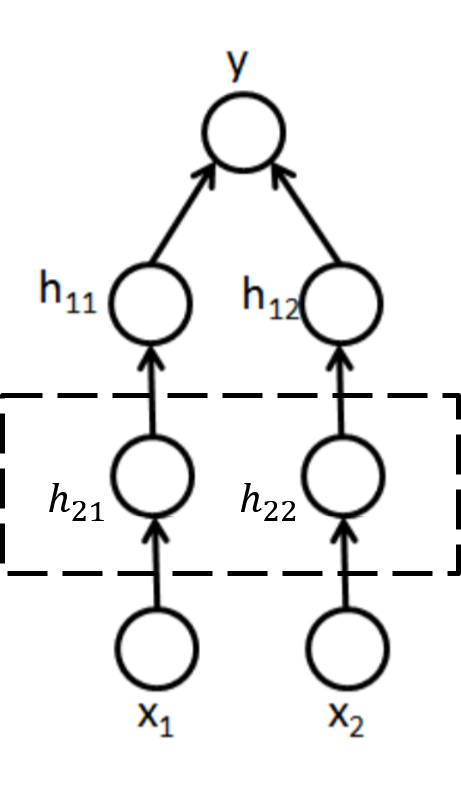
\includegraphics[width=0.25\linewidth]{fig/insert.png}
    \caption{\small
    new layer.}
    \label{fig:insert}
\end{figure}

Like in Figure~\ref{fig:insert},
we insert a layer above the input,
which contains two neurons
$h_{21}=f_{21}(x_1)$,
$h_{22}=f_{22}(x_2)$, and


\begin{equation}
    f_{21}(x_1) = \begin{cases}
            x_1, \quad\quad\quad \text{when }x_1\le 1, \\
            2-x_1, \quad \text{otherwise}.
        \end{cases}
\end{equation}
\begin{equation}
    f_{22}(x_2) := f_{21}(x_2).
\end{equation}
